% $> xelatex spsi.tor.presentacion.tex
% o bien
% $> lualatex spsi.tor.presentacion.tex
\documentclass[spanish,aspectratio=169]{beamer}

\usepackage[es-tabla]{babel}

% Tikz

\usepackage{graphics,tikz}
\usetikzlibrary{automata, positioning, arrows, fit, shapes}

\tikzset{
% ->, >=stealth,
% line width=2.75pt,
every path/.style={>=stealth, very thick, rounded corners},
state/.style={
rectangle, rounded corners,
draw=black, fill=gray!10, thick,
minimum height=2em, inner sep=10pt, text centered
}
}

\usepackage{pgfplotstable}
\pgfplotsset{compat=1.16}

\usepackage{adjustbox}
\usepackage{booktabs}
\usepackage{multirow}
\usepackage[inline]{enumitem}

%%% FUENTES

\usepackage[no-math]{fontspec}
\setmainfont{Inter}
\setsansfont{Inter}
\setmonofont{Roboto Mono}

%\usepackage{newtxsf}
\usepackage[math-style=TeX]{unicode-math}
\setmathfont{Fira Math}
\setmathfont[range=up/{num}]{Inter}
%\setmathfont[range=it/{greek,Greek}]{Inter Italic}
\setmathfont[range=it]{Inter Italic}
\setmathfont[range={cal, bb, frak, "22EE}, StylisticSet={3}, Scale=1.2]{Garamond Math}

\usepackage{pifont}
\newcommand{\cmark}{\ding{51}}%
\newcommand{\xmark}{\ding{55}}%

\usepackage{fontawesome5}
\usepackage{stackrel}

%%% COLORES

\definecolor{background}{HTML}{F5F5F4}
\definecolor{foreground}{HTML}{3F3F3F}
\definecolor{strings}{HTML}{ED982C}
\definecolor{operators}{HTML}{CF4818}
\definecolor{identifiers}{HTML}{9A71BA}
\definecolor{keywords}{HTML}{5486C8}
%\definecolor{keywords}{HTML}{54BFC7}
\definecolor{numbers}{HTML}{80951D}
\definecolor{comments}{HTML}{AFAFAF}

\definecolor{red}{HTML}{E64940}
\definecolor{green}{HTML}{2AA74D}
\definecolor{yellow}{HTML}{cc860c}
\definecolor{blue}{HTML}{2B76C3}

%%% LISTINGS

\usepackage{listings}

\lstset{
numbers=left,
belowcaptionskip=1\baselineskip,
basicstyle=\scriptsize\ttfamily\color{foreground},
keywordstyle=\color{blue},
commentstyle=\color{comments},
stringstyle=\color{strings},
%identifierstyle=\color{identifiers},
numberstyle=\color{foreground},
xleftmargin=2em,
framexleftmargin=1.5em,
breaklines=true,
showstringspaces=false,
tabsize=2,
escapeinside=çç,
morekeywords={sage},
moredelim=**[is][\color{red}]{@}{@},
}

% Algoritmo

\usepackage[linesnumbered, onelanguage]{algorithm2e}
\newcommand\mycommentfont[1]{\small\textcolor{foreground!70}{#1}}
\SetCommentSty{mycommentfont}

% Caption
\usepackage{caption}
\captionsetup[figure]{justification=raggedright,singlelinecheck=false}

\usepackage{tabularx}

%%% AJUSTES DE BEAMER

%\usefonttheme{professionalfonts}

\setlength{\leftmargini}{0.5cm}
%\setlength{\leftmarginii}{2em}

\setbeamertemplate{navigation symbols}{}

\setbeamerfont{title}{series=\bfseries, size=\Huge}
\setbeamerfont{date}{size=\small}
\setbeamerfont{institute}{size=\small}
\setbeamercolor{institute}{fg=foreground!80}
\setbeamercolor{date}{fg=foreground!80}

%\setbeamertemplate{frametitle}{\color{foreground}\vspace*{1cm}\bfseries\insertframetitle\par\vskip-6pt}
\setbeamerfont{frametitle}{series=\bfseries, size=\LARGE}
\setbeamercolor{frametitle}{fg=foreground}
\setbeamerfont{framesubtitle}{size=\normalfont\small}
\setbeamercolor{framesubtitle}{fg=foreground}

\setbeamercolor{background canvas}{bg=background}

\setbeamercolor{normal text}{fg=foreground}
\setbeamercolor{alerted text}{fg=foreground}
\setbeamercolor{block title}{fg=foreground}
\setbeamercolor{alerted text}{fg=foreground}

\setbeamercolor{itemize item}{fg=foreground}
\setbeamercolor{enumerate item}{fg=foreground}

\setbeamertemplate{itemize items}[circle]
\setitemize{
label=\usebeamerfont*{itemize item}
\usebeamercolor[fg]{itemize item}
\usebeamertemplate{itemize item}
}

\setbeamercolor*{title}{fg=foreground}
\setbeamercolor{qed symbol}{fg=foreground}

\usebeamercolor[fg]{normal text}

\setbeamertemplate{footline}[frame number]
% \setbeamertemplate{footline}[text line]{%
%   \parbox{\linewidth}{\color{foreground!60}\small\vspace*{-8pt}\insertsection\hfill\insertpagenumber}
% }
\setbeamerfont{page number in head/foot}{size=\small}

\setbeamercolor{section in toc}{fg=foreground}
\setbeamerfont{section in toc}{series=\bfseries}

\setbeamercolor{caption name}{fg=foreground}
\setbeamerfont{caption name}{series=\bfseries}

\setbeamercolor{bibliography entry note}{fg=foreground}
\setbeamercolor{bibliography entry author}{fg=foreground!40!black}

\setbeamertemplate{title page}[default][left]

\usefonttheme{structurebold}

\AtBeginSection[]{
\begin{frame}
  \vfill
  %\centering
  \raggedright
  \usebeamerfont{title}\Huge\insertsectionhead\par%
  \vfill
\end{frame}
}

\setlength{\parskip}{\baselineskip} 

\makeatletter
\setbeamertemplate{frametitle}{
\ifbeamercolorempty[bg]{frametitle}{}{\nointerlineskip}%
\@tempdima=\textwidth%
\advance\@tempdima by\beamer@leftmargin%
\advance\@tempdima by\beamer@rightmargin%
\hspace*{0.4cm}%%%%%%%%%%%%% For example insert shift to right
\begin{beamercolorbox}[sep=0.6cm,left,wd=\the\@tempdima]{frametitle}
  \usebeamerfont{frametitle}%
  \vbox{}\vskip-1ex%
  \if@tempswa\else\csname beamer@ftecenter\endcsname\fi%
  \strut\insertframetitle\strut\par%
  {%
  \ifx\insertframesubtitle\@empty%
  \else%
  {\usebeamerfont{framesubtitle}\usebeamercolor[fg]{framesubtitle}\insertframesubtitle\strut\par}%
  \fi
  }%
  \vskip-1ex%
  \if@tempswa\else\vskip-.3cm\fi% set inside beamercolorbox... evil here...
\end{beamercolorbox}%
}
\makeatother

\hypersetup{
colorlinks=true,
citecolor=numbers,
urlcolor=operators,
linkcolor=foreground
}

%%% INFORMACIÓN DEL DOCUMENTO

\title{Algoritmo de Peterson-Gorenstein-Zierler para códigos cíclicos sesgados}
%\subtitle{Trabajo de Fin de Grado}
\author{José María Martín Luque}
\institute{Universidad de Granada}
\date{9 de julio de 2020 - Curso 2019-2020}

\begin{document}

\maketitle

\begin{frame}{Índice}
  \tableofcontents
\end{frame}

\section{Introducción}

\begin{frame}{Transmisión de la información}
  \begin{figure}[h]
    \centering
    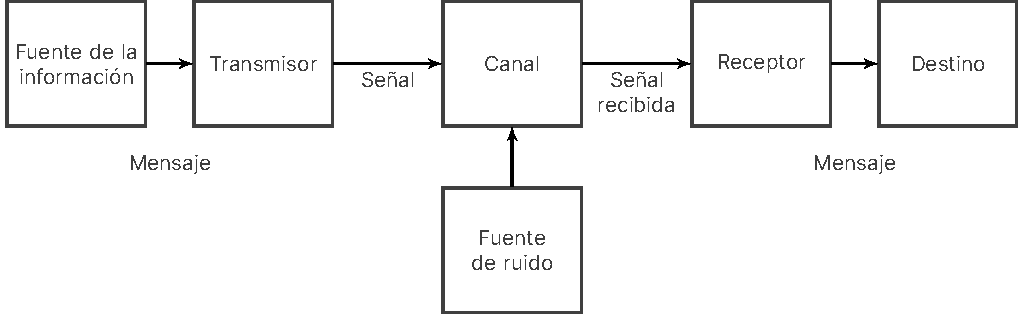
\includegraphics[width=\textwidth]{assets/shannon-communication-model}
    \caption{modelo de comunicación de Shannon}
  \end{figure}
\end{frame}

\begin{frame}{Transmisión de la información}
  
  Un código permite expresar información para su transmisión a través de un canal.
  
  El algoritmo de Peterson-Gorenstein-Zierler permite corregir errores producidos en la transmisión de información si se han usado ciertos códigos cíclicos.
  
\end{frame}

\begin{frame}{Objetivos}
  
  \begin{enumerate}
    \item Exponer y estudiar el algoritmo de Peterson-Gorenstein-Zierler para códigos cíclicos sesgados.
    \pause
    \begin{itemize}[label={\faArrowCircleRight}]
      \item Estudio de la teoría de códigos lineales.
      \item Estudio de la teoría de polinomios de Ore y sus cocientes.
    \end{itemize}
    \pause
    \item Implementar sistemas de decodificación en Python usando SageMath.
  \end{enumerate}
  
\end{frame}

\begin{frame}{Contenido}
  \color{foreground!60}
  \begin{description*}[font=\normalfont]
    \item[anillos]
    \item[ideales] 
    \item[cuerpos finitos] 
    \item[cuerpos de descomposición] 
    \item[elementos primitivos] 
    \item[clases ciclotómicas] 
    \item[anillos de polinomios] 
    \item[automorfismos] 
    \item[bases normales] 
    \item[\textbf{\textcolor{foreground}{códigos lineales}}]
    \item[\textbf{\textcolor{foreground}{códigos cíclicos}}]
    \item[códigos BCH]
    \item[PGZ para códigos BCH]
    \item[códigos RS]
    \item[idempotentes] 
    \item[\textbf{\textcolor{foreground}{anillos de polinomios de Ore}}]
    \item[\textbf{\textcolor{foreground}{códigos cíclicos sesgados}}]
    \item[\textbf{\textcolor{foreground}{PGZ para códigos RS sesgados}}]
  \end{description*}
  
\end{frame}

\section{Teoría de códigos}
\begin{frame}{¿Qué es un código?}
  \setbeamercolor{alerted text}{fg=red}
  \begin{definition}
    Un \((n, M)\) \emph{código} \(\mathcal C\) sobre el cuerpo \(\mathbb F_q\) es un subconjunto de tamaño \(M\) de \(\mathbb F_q^n\).
  \end{definition}
  
  Los elementos de un código se llaman \emph{palabras código}.
\end{frame}

\begin{frame}
  \frametitle{¿Qué es un código?}
  
  \begin{figure}[h]
    \centering
    \only<1>{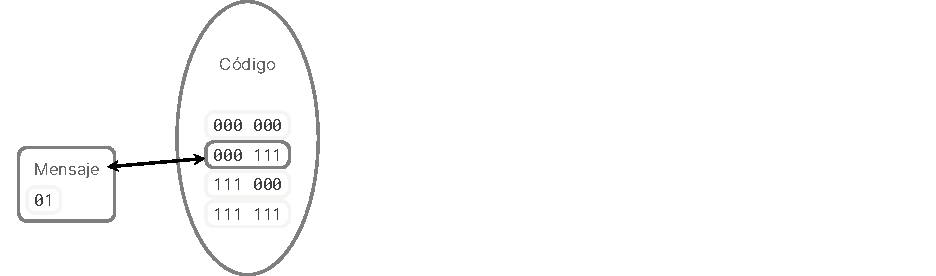
\includegraphics[width=\textwidth]{assets/diagrama-codigo1}}%
    \only<2>{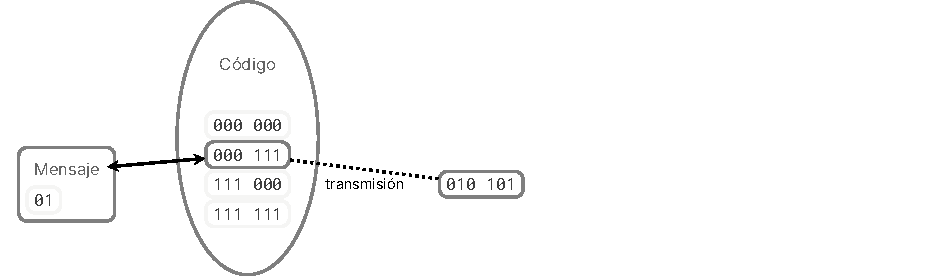
\includegraphics[width=\textwidth]{assets/diagrama-codigo2}}%
    \only<3>{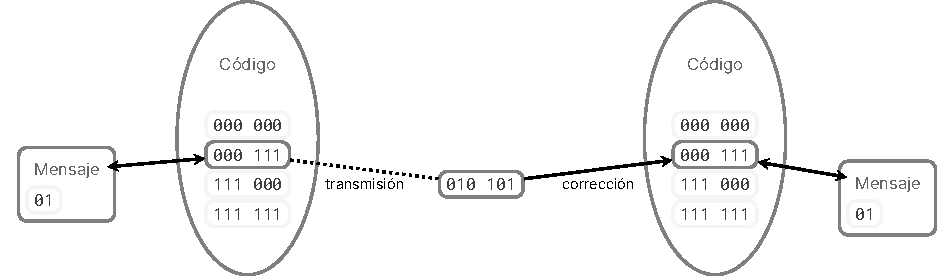
\includegraphics[width=\textwidth]{assets/diagrama-codigo3}}
    \caption{codificación y decodificación}
  \end{figure}
  
\end{frame}

\begin{frame}
  \frametitle{¿Qué es un código?}
  
  \setbeamercolor{alerted text}{fg=red}
  \begin{definition}
    Un \((n, M)\) \emph{código} \(\mathcal C\) sobre el cuerpo \(\mathbb F_q\) es un \alert{subconjunto} de \(\mathbb F_q^n\) de tamaño \(M\).
  \end{definition}
  
  Los elementos de un código se llaman \emph{palabras código}.
  
  \vspace{2em}
  \textcolor{red}{\faTimesCircle} Es un objeto demasiado sencillo.
  
\end{frame}

\begin{frame}{Añadiendo estructura}
  \setbeamercolor{alerted text}{fg=green}
  \begin{definition}
    Un \([n, k]\) \emph{código lineal \(\mathcal C\) de longitud \(n\) y dimensión \(k\)} es un \alert<2,3>{subespacio vectorial} de \(\mathbb F_q^n\) de dimensión \(k\).
  \end{definition}
  
  \pause
  
  \textcolor{green}{\faCheckCircle} Trabajamos con una estructura bien conocida.
  
  \pause
  
  \textcolor{green}{\faCheckCircle} Codificar es sencillo: multiplicar por una matriz (base).
\end{frame}

\begin{frame}{Añadiendo estructura}
  \setbeamercolor{alerted text}{fg=green}
  \begin{definition}
    Un código lineal \(\mathcal C\) de longitud \(n\) sobre \(\mathbb F_q\) es \textit{cíclico} si verifica:
    \[(c_0, \dots, c_{n-2}, c_{n-1}) \in \mathcal C \iff (c_{n-1}, c_0, \dots, c_{n-2}) \in \mathcal C\]
  \end{definition}
  
  \pause
  
  Podemos \alert<3,4>{asociar los elementos de \(\mathcal C\) a polinomios} mediante una biyección
  \begin{align*}
    \mathfrak v: \mathbb F_q^n &\to \mathbb F_q[x]/(x^n - 1)\\
    (c_0, c_1, \dots, c_{n-1}) &\mapsto c_0 + c_1x + \dots + c_{n-1}x^{n-1}.
  \end{align*}
  \pause
  \textcolor{green}{\faCheckCircle} Más estructura: los códigos cíclicos son ideales del cociente \(\mathbb F_q[x]/(x^n - 1)\).
  \pause
  \textcolor{green}{\faCheckCircle} Codificar es sencillo: multiplicar por un polinomio (generador del ideal).
\end{frame}

\begin{frame}{Distancia de un código}
  \begin{definition}
    La \emph{distancia de Hamming} de un código \(\mathcal C\) es el menor número de coordenadas que distinguen a una palabra código de otra.
  \end{definition}
\end{frame}

\section{Polinomios de Ore y códigos cíclicos sesgados}

\begin{frame}{Polinomios de Ore}
  \begin{definition}
    Sea \(\mathbb F_q\) un cuerpo finito y \(\sigma\) un automorfismo de \(\mathbb F_q\).
    Entonces, el anillo \(\mathbb F_q[x; \sigma]\) de los polinomios usuales de \(\mathbb F_q[x]\) cuyo producto verifica la relación:
    \[
    xa = \sigma(a)x,\qquad a \in \mathbb F_q,
    \]
    es un \textit{anillo de polinomios de Ore} o \textit{anillos de polinomios sesgados}.
  \end{definition}
\end{frame}

\begin{frame}{Polinomios de Ore}
  Es un anillo no conmutativo.
  
  Pero es un DIP y la aritmética funciona igual, teniendo en cuenta siempre que las operaciones se realizarán a izquierda o a derecha.
\end{frame}

\begin{frame}{Códigos cíclicos sesgados}
  Códigos cíclicos pero usando polinomios de Ore: 
  la biyección es \(\mathfrak v: \mathbb F_q^n \to \mathbb F_q[x; \sigma]/(x^n - 1)\), donde \(n\) es el orden de \(\sigma\).
  
  \pause
  
  \vspace{1cm}
  \begin{definition}
    Un \emph{código cíclico sesgado} sobre \(\mathbb F_q\) es un subespacio vectorial \(\mathcal C \subseteq \mathbb F_q^n\) tal que:
    %si \((a_0, \dots, a_{n-2}, a_{n-1}) \in \mathcal C\) entonces \((\sigma(a_{n-1}), \sigma(a_0), \dots, \sigma(a_{n-2})) \in \mathcal C\).
    \[(a_0, \dots, a_{n-2}, a_{n-1}) \in \mathcal C \iff (\sigma(a_{n-1}), \sigma(a_0), \dots, \sigma(a_{n-2})) \in \mathcal C\]
  \end{definition}
  
  \pause
  
  \begin{tabularx}{\textwidth}{@{}c@{\hskip 0.3em}X@{}}
    \textcolor{blue}{\faInfoCircle} &  Los códigos cíclicos sesgados son ideales del cociente \(\mathbb F_q[x; \sigma]/(x^n - 1)\).
  \end{tabularx}
\end{frame}

\begin{frame}{Códigos RS sesgados}
  Consideremos una base normal \(\{\alpha, \sigma(\alpha), \dots, \sigma^{n-1}(\alpha)\}\) de \(\mathbb F_q\) y \(\beta = \alpha^{-1}\sigma(\alpha)\).
  
  El monomio \(x - \beta\) divide a \(x^n - 1\) por la derecha, y de hecho
  \[
  x^n - 1 = \left[x - \beta, x - \sigma(\beta), \dots, x - \sigma^{n-1}(\beta)\right]_i.
  \]
  \pause
  
  \begin{tabularx}{\textwidth}{@{}c@{\hskip 0.3em}X@{}}
    \textcolor{blue}{\faInfoCircle} &  A los elementos de \(\{\beta, \sigma(\beta), \dots, \sigma^{n-1}(\beta)\}\) los llamamos \(\beta\)-\emph{raíces}.
  \end{tabularx}
\end{frame}

\begin{frame}{Códigos RS sesgados}
  \begin{definition}
    Un \emph{código RS sesgado} de distancia mínima diseñada \(\delta\) es un código cíclico sesgado \(\mathcal C\) tal que \(\mathfrak v(\mathcal C)\) está generado por 
    \[
    g = \left[x - \sigma^r(\beta), x - \sigma^{r+1}(\beta), \dots, x - \sigma^{r+\delta-2}(\beta)\right]_i
    \] 
    para algún \(r \geq 0\).
  \end{definition}
  \pause
  \begin{tabularx}{\textwidth}{@{}c@{\hskip 0.3em}X@{}}
    \textcolor{blue}{\faInfoCircle} & Tienen distancia \(\delta = n - k + 1\), máxima distancia posible para un código de esta longitud y dimensión.
  \end{tabularx}
\end{frame}

\begin{frame}{Norma}
  En un anillo \(\mathbb F_q[x; \sigma]\) definimos la \emph{norma} \(i\)\emph{-ésima} de un elemento \(\gamma \in \mathbb F_q\) como
  \[
  N_i(\gamma) = \sigma(N_{i-1}(\gamma))(\gamma) = \sigma^{i-1}(\gamma)\dots \sigma(\gamma)\gamma \quad\text{para } i > 0 \quad\text{y } N_0(\gamma) = 1.
  \]
  
  \pause
  
  \begin{tabularx}{\textwidth}{@{}c@{\hskip 0.3em}X@{}}
    \textcolor{blue}{\faInfoCircle} &  Es el equivalente a evaluar un polinomio en álgebra conmutativa.
  \end{tabularx}
  \vspace{0.6cm}
  
  \pause
  
  \begin{theorem}
    \label{prop:norma-divisor}
    Si \(f(x) = \sum_{i=0}^n a_ix^{n-i} \in \mathbb F_q[x; \sigma]\) y \(\gamma \in \mathbb F_q\) entonces el resto de dividir \(f(x)\) por \((x - \gamma)\) por la derecha es \[
    \sum_{i=0}^n a_iN_{i}(\gamma).
    \]
  \end{theorem}
\end{frame}

\begin{frame}{Norma}
  Sea \(N\) la matriz formada por las normas de las \(\beta\)-raíces:
  \[
  N = \begin{pmatrix}
    N_0(\beta) & N_0(\sigma(\beta)) & \cdots & N_0(\sigma^{n-1}(\beta))\\
    N_1(\beta) & N_1(\sigma(\beta)) & \cdots & N_1(\sigma^{n-1}(\beta))\\
    \vdots & \vdots & \ddots & \vdots\\
    N_{n-1}(\beta) & N_{n-1}(\sigma(\beta)) & \cdots & N_{n-1}(\sigma^{n-1}(\beta))
  \end{pmatrix}.
  \]
  Multiplicando los coeficientes de un polinomio por N, \((f_1, \dots, f_{n-1})N\) obtenemos todos los restos de dividir dicho polinomio por cada una de las \(\beta\)-raíces.
\end{frame}

\section{Algoritmo PGZ para códigos RS sesgados}

\begin{frame}{Recepción de mensajes}
  Un mensaje recibido puede expresarse como
  \[
  y(x) = c(x) + e(x)
  \]
  donde \(c(x)\) es el mensaje codificado original y \(e(x)\) es el error que se ha producido durante la transmisión, que es de la forma
  \[
  e(x) = e_{k_1}x^{k_1} + e_{k_2}x^{k_2} + \dots + e_{k_v}x^{k_v}.
  \]
  
  \pause
  
  \vspace{1em}

  \faArrowCircleRight~ El algoritmo encuentra el error \(e(x)\) para códigos RS sesgados.

  \faArrowCircleRight~ Puede corregir hasta \(t = \left\lfloor \frac{d - 1}{2} \right\rfloor\) errores.
  
\end{frame}

\begin{frame}{Algoritmo}
  \setbeamercovered{transparent}
  \begin{algorithm}[H]
    \DontPrintSemicolon
    \onslide<1>{
    \KwIn{el código \(\mathcal C\), el mensaje recibido \(y = (y_0, \dots, y_{n-1}) \in \mathbb F_q^n\) con no más de \(t\) errores}
    \KwOut{el error \(e = (e_0, \dots, e_{n-1})\) tal que \(y - e \in \mathcal C\)}
    }
    \onslide<2>{
    \tcp{Paso 1: calcular síndromes}
    \For{\(0 \leq i \leq 2t - 1\)}{
    $s_i \longleftarrow \sum_{j=0}^{n-1}y_jN_j(\sigma^i(\beta))$\;
    }
    \If{\(s_i = 0\) para todo \(0 \leq i \leq 2t - 1\)}{\Return{\(0\)}}
    }
  \end{algorithm}
\end{frame}

\begin{frame}{Algoritmo}
  \setbeamercovered{transparent}
  \begin{algorithm}[H]
    \DontPrintSemicolon
    \setcounter{AlgoLine}{6}
    \onslide<1>{
    \tcp{Paso 2: hallar polinomio localizador y las coordenadas de error}
    \(S^t \longleftarrow \left(\sigma^{-j}(s_{i+j})\sigma^i(\alpha)\right)_{0 \leq i \leq t, 0 \leq j \leq t -1}\)\;
    }
    \onslide<2>{
    Calcular
    \[
    \operatorname{mepc}(S^t) = \left( \begin{array}{@{}c|c@{}}
      I_{\mu} & \multirow{3}{*}{\(0_{(t+ 1)\times (t - \mu)}\)} \\\cline{1-1}
      a_0 \cdots a_{\mu -1 } & \\\cline{1-1}
      H' &
    \end{array}\right)
    \]\label{algl:pgz-sesgados-mpec-St}\;%\vspace*{-1.5em}\;% Reducimos un poco el espacio vertical
    }
    \onslide<3>{
    \(\rho = (\rho_0, \dots, \rho_{\mu}) \longleftarrow (-a_0, \dots, -a_{\mu-1}, 1)\) y \(\rho N \longleftarrow (\rho_0, \dots, \rho_{\mu}, 0, \dots, 0)N\)\;\label{algl:pgz-sesgados-rho}
    \(\{k_1, \dots, k_v\} \longleftarrow \) coordenadas igual a cero de \(\rho N\)\;\label{algl:pgz-sesgados-pos-error}
    }
    %\caption{Peterson-Gorenstein-Zierler para códigos cíclicos sesgados.}
    %\label{alg:pgz-sesgados}
  \end{algorithm}
\end{frame}

\begin{frame}{Algoritmo}
  \setbeamercovered{transparent}
  \begin{algorithm}[H]
    \DontPrintSemicolon
    \setcounter{AlgoLine}{10}
    \If{\(\mu \neq v\)}{\label{algl:pgz-sesgados-if}
    \onslide<1>{
    Calcular \[M_{\rho} \longleftarrow \begin{pmatrix}
      \rho_0 & \rho_1 & \dots & \rho_{\mu} & 0 & \dots & 0\\
      0 & \sigma(\rho_0) & \dots & \sigma(\rho_{\mu - 1}) & \sigma(\rho_{\mu}) & \dots & 0\\
      & & \ddots & & & \ddots & \\
      0 & \dots & 0 & \sigma^{n - \mu - 1}(\rho_0) & \dots & \dots & \sigma^{n - \mu - 1}(\rho_{\mu})
    \end{pmatrix}_{(n - \mu) \times n}\]\vspace*{-1.5em}\;% Reducimos un poco el espacio vertical
    }
    \onslide<2>{
    \(N_{\rho} \longleftarrow M_{\rho}N\)\;
    \(H_{\rho} \longleftarrow \operatorname{mepf}(N_{\rho})\)\;\label{algl:pgz-sesgados-mpec-Nrho}
    \(H' \longleftarrow\) la matriz obtenida al eliminar las filas de \(H_{\rho}\) distintas de \(\varepsilon_i\) para algún \(i\)\;\label{algl:pgz-sesgados-h-prima}
    }
    \onslide<3>{
    \(\{k_1, \dots, k_v\} \longleftarrow\) las coordenadas de las columnas igual a cero de \(H'\)\;
    }
    }
  \end{algorithm}
\end{frame}

\begin{frame}{Algoritmo}
  \framesubtitle{Cálculo de las magnitudes de error}
  \begin{theorem}
    \label{prop:pgz-sesgados-magnitudes-error}
    Las magnitudes de error \((e_{1}, \dots, e_{v})\) son las soluciones del sistema de ecuaciones lineales
    \[
    X \underbrace{
    \begin{pmatrix}
      \sigma^{k_1}(\alpha) & \sigma^{k_1 + 1}(\alpha) & \dots & \sigma^{k_1 + v - 1}(\alpha)\\ 
      \sigma^{k_2}(\alpha) & \sigma^{k_2 + 1}(\alpha) & \dots & \sigma^{k_2 + v - 1}(\alpha)\\ 
      \vdots & \vdots & \ddots & \vdots\\ 
      \sigma^{k_v}(\alpha) & \sigma^{k_v + 1}(\alpha) & \dots & \sigma^{k_v + v - 1}(\alpha)\\ 
    \end{pmatrix}
    }_{(\Sigma^{v-1})^T}
    = (\alpha s_0, \sigma(\alpha)s_1, \dots, \sigma^{v-1}(\alpha)s_{v-1}).
    \]
  \end{theorem}
\end{frame}

\begin{frame}{Algoritmo}
  \setbeamercovered{transparent}
  \begin{algorithm}[H]
    \DontPrintSemicolon
    \setcounter{AlgoLine}{17}
    \onslide<1>{
    \tcp{Paso 3: resolver el sistema de los síndromes, obteniendo las magnitudes de error}
    Encontrar \((x_1, \dots, x_v)\) tal que \((x_1, \dots, x_v)(\Sigma^{v-1})^T = (\alpha s_0, \sigma(\alpha)s_1, \dots, \sigma^{v-1}(\alpha)s_{v-1})\)\;\label{algl:pgz-sesgados-solucion-sistema}
    }
    \onslide<2>{
    \tcp{Paso 4: construir el error y devolverlo}
    \Return{\((e_0, \dots, e_{n-1})\) con \(e_i = x_i\) para \(i \in \{k_1, \dots, k_v\}\), cero en otro caso}\label{algl:pgz-sesgados-error}
    }
  \end{algorithm}
\end{frame}

\begin{frame}{Obtención del mensaje original}
  Obtenido el error podemso restárselo al mensaje recibido, de forma que
  \[
  c(x) = y(x) - e(x) \in \mathcal C
  \]
  es el mensaje decodificado.
\end{frame}



\section{Implementación en SageMath}

\begin{frame}{Clases desarrolladas}
  Se han implementado en SageMath: \begin{itemize}
    \item Un decodificador para códigos BCH usando el algoritmo PGZ.
    \item Los códigos cíclicos sesgados y los códigos RS sesgados.
    \item Un decodificador para códigos RS sesgados usando el algoritmo PGZ.
  \end{itemize}
  
  Aprovechan la estructura de códigos de Sage y su uso es similar a las incluidas.
\end{frame}

\begin{frame}
  \Huge \emph{\textbf{Ejemplo}}
  
  \LARGE Implementación en SageMath
\end{frame}

\section{Conclusiones}

\begin{frame}{Conclusiones}
  
  \begin{itemize}
    \item Objetivos:
    \begin{itemize}[label=\textcolor{green}{\faCheckSquare}]
      \item Estudio de polinomios de Ore, códigos cíclicos sesgados y del algoritmo PGZ.
      \item Implementación en SageMath.
    \end{itemize}
    \item Posible trabajo futuro: completar implementación códigos cíclicos sesgados y contruibuir lo desarrollado al proyecto SageMath.
  \end{itemize}
\end{frame}

\begin{frame}
  \Huge Gracias por su atención
\end{frame}

\end{document}
